\documentclass{dsekprotokoll}
\usepackage[T1]{fontenc}
\usepackage[utf8]{inputenc}
\usepackage[swedish]{babel}
\usepackage{float}
\usepackage{booktabs}
\usepackage{array}

\setheader{Policy för Marknadsföring och Prissättning}{Policydokument}{Lund -- 9 September 2021}

\title{Policy för Marknadsföring och Prissättning}
\author{David Jobrant, Victor Winkelmann}

\begin{document}
\maketitle
\section{Formalia}
\subsection{Sammanfattning}
Policyn beskriver prissättning av olika former av marknadsföring D-sektionen erbjuder företag och andra organisationer.

\subsection{Syfte}
Syftet med denna policy är att tydliggöra prissättning för marknadsföring genom sektionens kanaler. Policyn baseras på företagets eller organisationens ekonomiska status samt studentnyttan för sektionens medlemmar.

\subsection{Omfattning}
Riktlinjerna är gällande för D-sektionens informationskanaler.

\subsection{Ägande}
Styrelsen äger policyn i sin helhet och har rätt att behandla och ändra denna på styrelsemöten.

\subsection{Historik}
Utkast färdigställt av David Jobrant, Informationsansvarig 21/22, Victor Winkelmann, Näringslivsansvarig 21/22. \\
Antagen på VTM 2021.
Uppdaterad enl. Policy för Policyer på HTM2 2021.

\section{Riktlinjer för Marknadsföring genom sektionens kanaler}
Inlägg relaterade till marknadsföring från företag bör ej överskrida tre gånger i veckan.

Annonser och marknadsföring från företag publiceras endast från Facebook-sidan 'Näringslivsutskottet D-sektionen inom TLTH'.

För andra fall som berör informationsspridning, se policyn 'Policy för informationsspridning genom sektionens kanaler".

\section{Priser och Betalning}

\subsection{Priskategori}

D-sektionen tillämpar tre olika priskategorier på informationskanalerna för att ta hänsyn till olika företags och organisationers förutsättningar.
Rabattsatserna appliceras på informationsspridning.

\begin{itemize}
    \item Priskategori 1: Gratis
    \item Priskategori 2: 50\% rabatt
    \item Priskategori 3: Fullpris
\end{itemize}
% \usepackage{booktabs}


\begin{table}[hbp!]
    \begin{tabular}{@{}lccc@{}}
        \toprule
                                           & \textbf{Näringslivsrelaterat} & \begin{tabular}[c]{@{}c@{}}\textbf{Studentnytta för }\\\textbf{TLTHs medlemmar }\end{tabular} & \begin{tabular}[c]{@{}c@{}}\textbf{Övrig }\\\textbf{marknadsföring }\end{tabular} \\
        \midrule
        \addlinespace
        \textbf{Företag, organisationer}   &                               &                                                                                               &                                                                                   \\
        \addlinespace
        \cmidrule{1-1}
        Vinstdrivande                      & 3                             & 3                                                                                             & 3                                                                                 \\
        Startup-företag                    & Fall till fall                & Fall till fall                                                                                & Fall till fall                                                                    \\
        Fackföreningar                     & 3                             & 3                                                                                             & 3                                                                                 \\
        Övriga ideella organisationer*     & 2                             & 1                                                                                             & 1                                                                                 \\
        \addlinespace
        \midrule
        \addlinespace
        \textbf{Studentföreningar}         &                               &                                                                                               &                                                                                   \\
        \addlinespace
        \cmidrule{1-1}
        Teknologkårens centralorganisation & -                             & 1                                                                                             & 1                                                                                 \\
        Sektioner, Intresseföreningar      & -                             & 1                                                                                             & 1                                                                                 \\
        Fria föreningar inom TLTH          & -                             & 1                                                                                             & 1                                                                                 \\
        LUS, SFS                           & -                             & 1                                                                                             & 1                                                                                 \\
        Akademiska Föreningen              & 2                             & 2                                                                                             & 2                                                                                 \\
        Studentlunds centralorganisation   & 2                             & 1                                                                                             & 2                                                                                 \\
        Nationer                           & 2                             & 2                                                                                             & 2                                                                                 \\
        Övriga studentorganisationer       & 2                             & 1                                                                                             & 2                                                                                 \\
        \addlinespace
        \midrule
        \addlinespace
        \textbf{Lunds Universitet}         &                               &                                                                                               &                                                                                   \\
        \addlinespace
        \cmidrule{1-1}
        LTH                                & 2                             & 1                                                                                             & 1                                                                                 \\
        Övriga LU                          & 2                             & 1                                                                                             & 2                                                                                 \\
        \addlinespace
        \bottomrule
    \end{tabular}
\end{table}


% \begin{figure}[H]
%     \centering
%     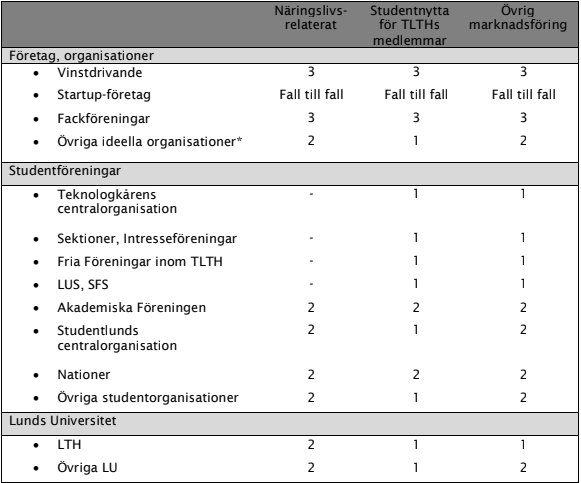
\includegraphics[scale=1]{marknadsforing_1.png}
%     \caption{Informationskanalernas priskategorier för olika företag och organisationer }
%     \label{fig5}
% \end{figure}

*Med övriga ideella organisationer menas de organisationer som inte bedriver verksamhet  som vi har och som inte är studentföreningar.

Samma priskategorier kan appliceras med fördel på event och aktiviteter. Dock behandlas eventförfrågningar från fall till fall där Näringslivsansvarig, samt Näringslivsutskottet, bedömer omständigheterna och förutsättningar från organisationen som  skickat förfrågan.

\subsection{Specialfall}
Specialfall, då mindre vanliga, speciella förfrågningar eller dylikt inkommer som inte täcks av  ovan punkter bedöms de fallen från fall till fall. Näringslivsansvarig och Informationsansvarig har i de fallen bestämmanderätt.

\end{document}